\documentclass[t]{beamer}
\usetheme{Copenhagen}
\setbeamertemplate{headline}{} % remove toc from headers
\beamertemplatenavigationsymbolsempty

\usepackage{amsmath, array, tikz, bm, pgfplots, tcolorbox, graphicx, venndiagram, color, colortbl, xfrac}
\pgfplotsset{compat = 1.16}
\usepgfplotslibrary{statistics}
\usetikzlibrary{calc}

\title{Hypothesis Testing}
\subtitle{Single Sample Proportion}
\author{}
\date{}

\AtBeginSection[]
{
  \begin{frame}
    \frametitle{Objectives}
    \tableofcontents[currentsection]
  \end{frame}
}

\begin{document}

\pgfmathdeclarefunction{gauss}{2}{%
  \pgfmathparse{1/(#2*sqrt(2*pi))*exp(-((x-#1)^2)/(2*#2^2))}%
}

\begin{frame} 
\maketitle
\end{frame}

\begin{frame}{Testing a Population Proportion}
In this section, we will test a claim regarding a population proportion. \newline\\ \pause

\textbf{Assumptions}
\begin{itemize}
\item<3->{A random sample is selected from a binomial population (\textit{success or failure})}	\newline\\
\item<4->{The sample size $n$ is large}
\begin{itemize}
	\item<5->{Will be met if $np$ and $n(1-p)$ are each at least 15}
\end{itemize}
\end{itemize}
\end{frame}
\begin{frame}{Test Statistic and Standard Error}
The sample proportion, $\hat{p}$ is given by	\bigskip
\[\hat{p} = \frac{x}{n} = \frac{\text{number of observed successes}}{\text{sample size}}\]		\newline\\	\pause
with sample standard error	
\[\sigma_{\hat{p}} = \sqrt{\frac{\hat{p}(1-\hat{p})}{n}}\]
\end{frame}

\begin{frame}{Test Statistic and Critical Value Method}
The test statistic of the population proportion, $z$, can be found by calculating
\begin{align*}
z &= \frac{\hat{p} - p}{\sqrt{p(1-p)/n}} \\[10pt]
\onslide<2->{&= \frac{\text{sample proportion}-\text{population proportion}}{\text{standard error}}} \\
\end{align*}
\begin{center}
\onslide<3->{
\begin{tabular}{c|c}
\textbf{Significance Level} & \textbf{Critical Value} \\ \hline
$\alpha = 0.01$ & $\pm 2.576$ \\
$\alpha = 0.05$ & $\pm 1.96$  \\
$\alpha = 0.10$ & $\pm 1.645$ \\
\end{tabular}
}
\end{center}
\end{frame}

\begin{frame}{Test Statistic and Critical Value Method}
\begin{center}
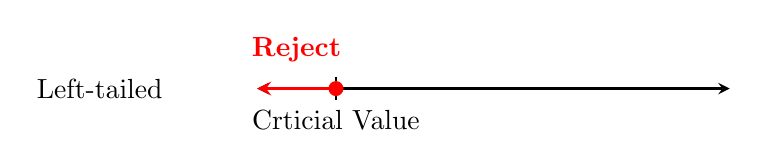
\begin{tikzpicture}[>=stealth]
\node at (-5,0) {Left-tailed};
\draw[<->, thick] (-3,0) -- (3,0);
\draw (-2,0.15) -- (-2,-0.15) node [below] {Crticial Value};
\draw [color=red, fill=red] (-2,0) circle [radius=2.5pt];
\draw[->, color=red, very thick] (-2,0) -- (-3,0);
\node at (-2.5,0.5) [color=red] {\textbf{Reject}};
\end{tikzpicture}
\newline\\
\onslide<2->{
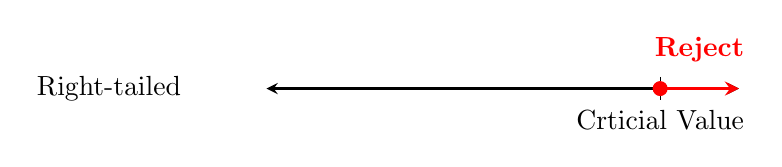
\begin{tikzpicture}[>=stealth]
\node at (-5,0) {Right-tailed};
\draw[<->, thick] (-3,0) -- (3,0);
\draw (2,0.15) -- (2,-0.15) node [below] {Crticial Value};
\draw [color=red, fill=red] (2,0) circle [radius=2.5pt];
\draw[->, color=red, very thick] (2,0) -- (3,0);
\node at (2.5,0.5) [color=red] {\textbf{Reject}};
\end{tikzpicture}}
\newline\\
\onslide<3->{
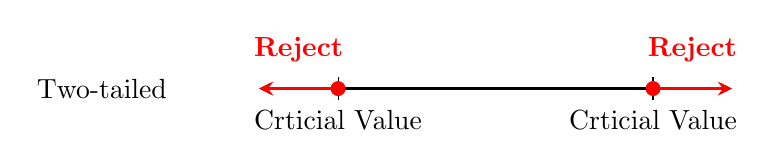
\begin{tikzpicture}[>=stealth]
\node at (-5,0) {Two-tailed};
\draw[<->, thick] (-3,0) -- (3,0);
\draw (-2,0.15) -- (-2,-0.15) node [below] {Crticial Value};
\draw [color=red, fill=red] (-2,0) circle [radius=2.5pt];
\draw[->, color=red, very thick] (-2,0) -- (-3,0);
\node at (-2.5,0.5) [color=red] {\textbf{Reject}};
\draw (2,0.15) -- (2,-0.15) node [below] {Crticial Value};
\draw [color=red, fill=red] (2,0) circle [radius=2.5pt];
\draw[->, color=red, very thick] (2,0) -- (3,0);
\node at (2.5,0.5) [color=red] {\textbf{Reject}};
\end{tikzpicture}}
\end{center}
\end{frame}

\begin{frame}{$p$-Value Method}
The area of the rejection region is given by $\alpha$, the significance level. \newline\\	\pause

Recall that the $p$-value is the probability of obtaining sample results as extreme (or more) than one we got. \newline\\	\pause

If our $p$-value is lower than $\alpha$, then our results are {\color{blue}\textbf{statistically significant}}, and would not likely occur by chance if the null hypothesis were true.	\newline\\	\pause

Reminder, if the $p\text{-value} < \alpha$, we reject the null hypothesis.
\end{frame}

\begin{frame}{$p$-Value Method}
\begin{center}
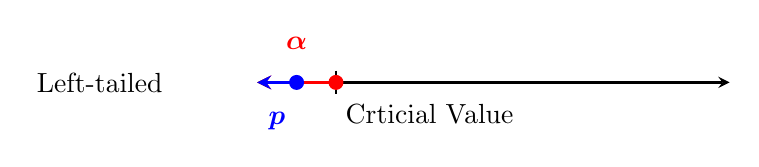
\begin{tikzpicture}[>=stealth]
\node at (-5,0) {Left-tailed};
\draw[<->, thick] (-3,0) -- (3,0);
\draw (-2,0.15) -- (-2,-0.15) node [below right] {Crticial Value};
\draw [color=red, fill=red] (-2,0) circle [radius=2.5pt];
\draw[->, color=red, very thick] (-2,0) -- (-3,0);
\node at (-2.5,0.5) [color=red] {$\bm{\alpha}$};
\onslide<2->{
\draw [color=blue, fill=blue] (-2.5,0) circle [radius=2.5pt];
\draw[->, color=blue, very thick] (-2.5,0) -- (-3,0);
\node at (-2.75,-0.25) [below, color=blue] {$\bm{p}$};
}
\end{tikzpicture}
\newline\\
\onslide<3->{\textbf{Reject null}}	\vspace{1cm}
\onslide<4->{
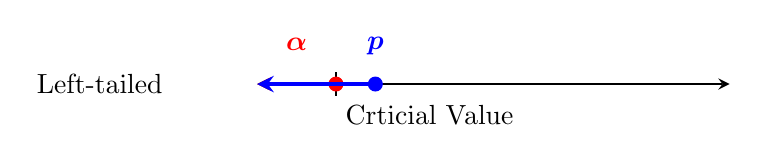
\begin{tikzpicture}[>=stealth]
\node at (-5,0) {Left-tailed};
\draw[<->, thick] (-3,0) -- (3,0);
\draw (-2,0.15) -- (-2,-0.15) node [below right] {Crticial Value};
\draw [color=red, fill=red] (-2,0) circle [radius=2.5pt];
\draw[->, color=red, very thick] (-2,0) -- (-3,0);
\node at (-2.5,0.5) [color=red] {$\bm{\alpha}$};
\onslide<5->{
\draw[->, color=blue, ultra thick] (-1.5,0) -- (-3,0);
\draw [color=blue, fill=blue] (-1.5,0) circle [radius=2.5pt];
\node at (-1.5,0.25) [above, color=blue] {$\bm{p}$};
}
\end{tikzpicture}}
\newline\\
\onslide<6->{\textbf{Do Not Reject Null}}
\end{center}
\end{frame}

\begin{frame}{Confidence Interval Method}
Our confidence interval for a population proportion is given by 

\[\text{point estimate} \pm \text{margin of error}\] 
\onslide<2->{\[\hat{p} \pm z_{\alpha/2}\sqrt{\frac{\hat{p}(1-\hat{p})}{n}}\]}	\newline\\
\onslide<3->{If our confidence interval contains the (claimed) population proportion, we do not reject the null hypothesis.}	\newline\\

\onslide<4->{For one-sided testing, use the critical value $z_{\alpha}$.}
\end{frame}

\begin{frame}{Confidence Interval Method}
\begin{center}
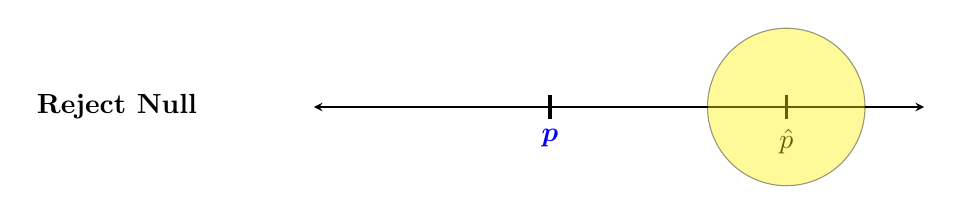
\begin{tikzpicture}[>=stealth]
\node at (-6.5,0) {\textbf{Reject Null}};
\draw[<->] (-4,0) -- (3.75,0);
\draw [very thick] (-1,0.15) -- (-1,-0.15) node [below, color=blue] {$\bm{p}$};
\draw [very thick] (2,0.15) -- (2,-0.15) node [below] {$\hat{p}$};
\draw [fill=yellow, opacity = 0.4] (2,0) circle [radius = 1cm];
\end{tikzpicture}
\newline\\
\onslide<2->{
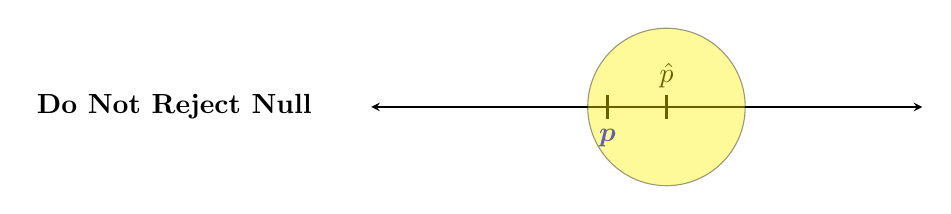
\begin{tikzpicture}[>=stealth]
\node at (-6.5,0) {\textbf{Do Not Reject Null}};
\draw[<->] (-4,0) -- (3,0);
\draw [very thick] (-1,0.15) -- (-1,-0.15) node [below, color=blue] {$\bm{p}$};
\draw [very thick] (-0.25,0.15) -- (-0.25,-0.15) node [above, yshift=0.25cm] {$\hat{p}$};
\draw [fill=yellow, opacity = 0.4] (-0.25,0) circle [radius = 1cm];
\end{tikzpicture}
}
\end{center}
\end{frame}

\begin{frame}{Example 1}
According to a recent study, 72\% of Americans favor starting school after Labor Day. You believe the percentage is greater than 72\%, so you obtain a sample of 400 Americans and find that 75\% of them favor starting school after Labor Day. \newline\\

At the $\alpha = 0.05$ significance level, test the claim.	\newline\\	\pause

$H_0: \, p = 0.72$ \newline
$H_A: \, p > 0.72$
\end{frame}

\begin{frame}{Example 1}
Test statistic: $z = 1.336$ (Critical Value = 1.645) \newline
$p$-value = 0.0907\newline
95\% lower bound: 0.7144	 \newline
(we are 95\% confident the population proportion is 71.44\% or higher)	\newline\\	\pause

Do not reject null hypothesis	\newline\\	\pause

\begin{quote}
At the 5\% significance level, we do not have sufficient evidence to reject the null hypothesis and conclude that our sample does not support the claim that the mean percentage of Americans who favor starting school after Labor Day is greater than 72\%.
\end{quote}
\end{frame}

\begin{frame}{Example 2}
According to a recent poll, 40\% of people would vote for Bryan Bain to be President of the United States (never going to happen). You want to test the claim (at the $\alpha = 0.05$ significance level) that the percent of people who would vote for Bryan Bain is not 40\%, so you obtain a random sample of 700 voters and find that 45\% would vote for Bryan Bain.	\newline\\

\onslide<2->{$H_0: \, p = 0.40$} \newline
\onslide<2->{$H_A: \, p \neq 0.40$}
\end{frame}

\begin{frame}{Example 2}
Test statistic: $z = 2.700$ (Critical value = 1.96)	\newline
$p$-value = 0.0069	\newline
Confidence Interval = (0.4131, 0.4869) \newline\\	\pause

Reject the null hypothesis.	\newline\\	\pause

\begin{quote}
At the 5\% significance level, we have sufficient evidence to reject the null hypothesis that the percentage of voters that would vote for Bryan Bain is 40\% and conclude that our sample supports the claim that the percentage may be different than 40.
\end{quote}
\pause

*On a personal note, take a look at any US President when they begin their first term and then see what they look like when they leave office. \emph{That} is why I don't want to be President.
\end{frame}

\end{document}